\documentclass[10pt,aspectratio=1610]{beamer}
\usetheme[height=1.5cm]{Rochester}
\definecolor{aqours}{HTML}{00A1E9}
\definecolor{chika}{HTML}{FF791B}
\definecolor{riko}{HTML}{FF7777}
\definecolor{kanan}{HTML}{00D29E}
\definecolor{dia}{HTML}{F43232}
\definecolor{you}{HTML}{2AA4DB}
\definecolor{yohane}{HTML}{AEAEAE}
\definecolor{hanamaru}{HTML}{CFBA0F}
\definecolor{mari}{HTML}{A530E0}
\definecolor{ruby}{HTML}{EE55B7}
\usecolortheme[named=aqours]{structure}

\usetheme[height=1.5cm]{Rochester}
\usecolortheme{seahorse}

\usefonttheme{structurebold}
\usefonttheme{serif}
\setbeamertemplate{navigation symbols}{}
\setbeamertemplate{items}[ball]
\setbeamertemplate{section in toc}[ball]
\setbeamertemplate{footline}[text line]{\parbox{\linewidth}{\vspace{-2em}\hfill\scriptsize\insertpagenumber}}
\setbeamertemplate{caption}[numbered]
\setbeamerfont{items}{size=\large}
\setlength{\parskip}{1.25em}
\linespread{1.25}

\AtBeginSection[]
{
  \begin{frame}
    \frametitle{\thesection. \secname}
    \tableofcontents[currentsection]
  \end{frame}
}

\usepackage{amsmath}
\usepackage{anyfontsize}
\usepackage{fontspec}
\usepackage{newpxtext}
\usepackage{newpxmath}
\setmonofont{Luxi Mono}

\usepackage{graphicx}
\usepackage{subcaption}
\usepackage{caption}
\captionsetup{font=scriptsize}
\usepackage{hyperref}
\hypersetup{
    colorlinks=true,
    linkcolor=dia,
    filecolor=yohane,
    urlcolor=kanan,
    citecolor=hanamaru,
}
\usepackage{tabularray}
\UseTblrLibrary{booktabs}
\usepackage{tikz}
\usetikzlibrary{calc,positioning,shapes.misc,arrows.meta}
\usepackage{setspace}

\usepackage[fontset=none]{ctex}
\setCJKmainfont{Source Han Serif CN Medium}[BoldFont=Source Han Serif CN Bold,ItalicFont=STKaiti,SmallCapsFont=STKaiti]
\setCJKsansfont{Source Han Serif CN Medium}[BoldFont=Source Han Serif CN Bold,ItalicFont=STKaiti,SmallCapsFont=STKaiti]
\setCJKmonofont{Source Han Sans CN}
\newCJKfontfamily\kaishu{STKaiti}[BoldFont=STKaiti]
\setbeamerfont{author}{family=\kaishu}
\setbeamerfont{date}{family=\kaishu}

\usepackage[backend=biber,sorting=none,style=authoryear,maxcitenames=2]{biblatex}
\addbibresource{reference.bib}
\defbibheading{bibliography}[\bibname]{}
\DeclareDelimFormat{finalnamedelim}{
    \ifnumgreater{\value{liststop}}{2}{\finalandcomma}{}
    \addspace\&\space}

\title{恒星演化的归宿}
\author{国家天文台 张植竣}
\date{2026年2月26日}

\begin{document}

\begin{frame}[plain]
    \maketitle
\end{frame}

\begin{frame}{目录}
    \tableofcontents
\end{frame}

\section{恒星演化的终局}

\begin{frame}{恒星演化概貌}
    \begin{figure}[!ht]
    \centering
    \begin{tikzpicture}[>=Stealth,node distance=0.75cm,main/.style={rectangle,minimum size=0.75cm,very thick,draw=structure.fg!50!white,top color=structure.fg!20!white,bottom color=structure.fg!20!white},test/.style={rounded rectangle,minimum size=0.75cm,very thick,draw=structure.fg!50!white,top color=white,bottom color=white,text=mari}]
        \node (O) [main] {分子云};
        \node (A) [main,below=of O] {原恒星};
        \draw [->,thick,double,structure.fg!50!white] (O.south) -- (A.north)
            node [midway,right,align=center] {\textit{引力坍缩}};
        \node (B) [main,below=of A] {主序星};
        \draw [->,thick,double,structure.fg!50!white] (A.south) -- (B.north)
            node [midway,right,align=center] {\textit{点燃氢核聚变}};
        \node (C1) [main,below left=of B] {超新星};
        \node (C2) [main,below right=of B] {行星状星云};
        \draw [->,thick,double,structure.fg!50!white] (B.south) -- (C1.north)
            node [midway,above left,align=center] {\textit{引力坍缩}};
        \draw [->,thick,double,structure.fg!50!white] (B.south) -- (C2.north)
            node [midway,above right,align=center] {\textit{热脉动}};
        \node (D1) [test,below left=of C1] {\textbf{黑洞}};
        \node (D2) [test,below right=of C1] {\textbf{中子星}};
        \node (D3) [test] at (C2 |- D1) {\textbf{白矮星}};
        \draw [->,thick,double,structure.fg!50!white] (C1.south) -- (D1.north);
        \draw [->,thick,double,structure.fg!50!white] (C1.south) -- (D2.north);
        \draw [->,thick,double,structure.fg!50!white] (C2.south) -- (D3.north);
    \end{tikzpicture}
    \end{figure}
\end{frame}

\begin{frame}{恒星演化的归宿}
    恒星\textcolor{mari}{如何演化}很大程度上取决于其\textcolor{dia}{初始质量}。以\textcolor{dia}{$8 M_\odot$}和\textcolor{dia}{$25 M_\odot$}为界，分别是形成\textcolor{mari}{白矮星}、\textcolor{mari}{中子星}和\textcolor{mari}{黑洞}的临界值。

    \begin{table}
    \centering
    \begin{tabular}{ccc}
    \toprule
    \textbf{初始质量（$M_\odot$）} & \textbf{氦核心质量（$M_\odot$）} & \textbf{演化结局} \\
    \midrule
    $< 0.08$ & - & 褐矮星 \\
    $0.08 \sim 0.5$ & - & He白矮星 \\
    $0.5 \sim 2.3$ & $< 0.45$ & 氦闪 $\to$ CO白矮星 \\
    $2.3 \sim 6$ & $0.45 \sim 1.9$ & CO白矮星（不经过氦闪） \\
    $6 \sim 8$ & $1.9 \sim 2.1$ & ONeMg白矮星 \\
    $8 \sim 25$ & $2.1 \sim 8$ & 中子星 \\
    $> 25$ & $> 8$ & 黑洞 \\
    \bottomrule
    \end{tabular}
    \end{table}
\end{frame}

\section{白矮星}

\begin{frame}{白矮星}
    \textcolor{dia}{白矮星}是恒星演化的最终阶段之一，通常是质量较小的恒星（初始质量小于约$8 M_\odot$）在经历了主序星阶段和红巨星阶段后形成的。白矮星没有核聚变来产生能量，微弱的亮度来自储存的能量的热辐射，其表面温度在$10^4\,\mathrm{K}$左右。

    白矮星的核心主要由碳和氧组成，外层可能有一层氦或氢包层。质量更大的白矮星会由氧、氖、镁组成。白矮星的密度非常高，通常在$10^6 \sim 10^9\,\mathrm{g/cm^3}$范围内。

    白矮星的稳定性主要依赖于\textcolor{dia}{电子简并压}，这是由量子力学效应引起的一种压力，可以抵抗引力坍缩，使得白矮星能够维持稳定状态。
\end{frame}

\begin{frame}{电子简并压}
    电子简并压是由泡利不相容原理引起的量子力学效应。

    \textcolor{dia}{泡利不相容原理}：\textcolor{mari}{两个或更多的费米子（如电子）不能占据同一量子态。}对于每一个能级，最多只能有\textcolor{mari}{两个电子（自旋向上和自旋向下）}。

    当一个恒星的核心坍缩时，电子被压缩到一个非常小的体积中。由于泡利不相容原理，电子不能占据同一量子态，因此它们必须占据更高的动量态。这种动量的增加产生了一个压力，称为\textcolor{dia}{电子简并压}，它抵抗进一步的压缩。

    我们日常生活中也有电子简并压的例子，比如在金属中，自由电子的简并压使得金属具有一定的硬度。
\end{frame}

\begin{frame}{电子简并压的推导：从不确定性原理开始}
    \textcolor{dia}{不确定性原理（测不准原理）}是量子力学的一个基本原理，表明\textcolor{mari}{我们不能同时精确地知道一个粒子的位置和动量}。对于一个粒子，我们有以下关系：
    \textcolor{mari}{
    \[
        \Delta x \Delta p \gtrsim h
    \]
    }
    其中$\Delta x$是位置的不确定性，$\Delta p$是动量的不确定性，$h$是普朗克常数。

    对于某个给定的$\Delta x$，这意味着：
    \[
        \Delta p \gtrsim \frac{h}{\Delta x}
    \]
    这表明当粒子被限制在一个非常小的空间中时，它的动量不确定性必须增加，从而导致动量的增加。
\end{frame}

\begin{frame}{电子简并压的推导：从不确定性原理开始}
    考虑$N$个电子被压缩到体积$V$中，电子密度为$n = \dfrac{N}{V}$。则每个电子占据的平均体积为$\dfrac{V}{N} = \dfrac{1}{n}$。因此，位置的不确定性可以估计为：
    \[
        \Delta x \sim n^{-1/3}
    \]
    根据不确定性原理，动量的不确定性为：
    \textcolor{dia}{
    \[
        \Delta p \gtrsim h n^{1/3}
    \]
    }
    这表明\textcolor{dia}{每个电子的动量正比于$n^{1/3}$}，因此电子的密度增加会导致动量的增加，从而产生更大的简并压。
\end{frame}

\begin{frame}{电子简并压的推导：费米球}
    \begin{minipage}{0.7\textwidth}
        更精确的推导涉及到电子在动量空间中的分布。根据不确定性原理，在三维空间中，电子的位置和动量会占据一定的\textcolor{mari}{相空间}，满足：
        \[
            (\Delta x \Delta y \Delta z) \cdot (\Delta p_x \Delta p_y \Delta p_z) = V_x \cdot V_p = h^3
        \]
        也就是说，如果电子的空间体积占据了$V_x$，那么在\textcolor{mari}{动量空间}中，每个电子占据的体积为：
        \[
            V_p = \frac{h^3}{V_x}
        \]
        在一个由$N$个电子组成的系统中，电子会从最低能量态逐级占据量子态。由于泡利不相容原理，每个量子态最多只能有两个电子（自旋向上和自旋向下）。由于系统的电子数是有限的，电子的动量存在一个最大值\textcolor{dia}{$p_F$}，称为\textcolor{dia}{费米动量}。
    \end{minipage}
    \begin{minipage}{0.29\textwidth}
        \begin{figure}
            \centering
            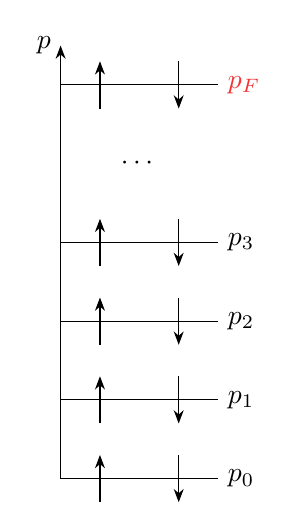
\begin{tikzpicture}[>=Stealth]
                \draw[->] (0,0) -- (0,5.5) node [left] {$p$};
                \draw (0,0) -- (2,0) node [right] {$p_0$};
                \draw [->] (0.5,-0.3) -- (0.5,0.3);
                \draw [<-] (1.5,-0.3) -- (1.5,0.3);
                \draw (0,1) -- (2,1) node [right] {$p_1$};
                \draw [->] (0.5,0.7) -- (0.5,1.3);
                \draw [<-] (1.5,0.7) -- (1.5,1.3);
                \draw (0,2) -- (2,2) node [right] {$p_2$};
                \draw [->] (0.5,1.7) -- (0.5,2.3);
                \draw [<-] (1.5,1.7) -- (1.5,2.3);
                \draw (0,3) -- (2,3) node [right] {$p_3$};
                \draw [->] (0.5,2.7) -- (0.5,3.3);
                \draw [<-] (1.5,2.7) -- (1.5,3.3);
                \node at (1,4) {$\cdots$};
                \draw (0,5) -- (2,5) node [right] {\textcolor{dia}{$p_F$}};
                \draw [->] (0.5,4.7) -- (0.5,5.3);
                \draw [<-] (1.5,4.7) -- (1.5,5.3);
            \end{tikzpicture}
        \end{figure}
    \end{minipage}
\end{frame}

\begin{frame}{电子简并压的推导：费米球}
        电子在\textcolor{mari}{动量空间}中会填充到一个称为\textcolor{dia}{费米球}的区域中。如图，其半径即为\textcolor{dia}{费米动量}。这是\textcolor{mari}{系统中电子最高允许的动量}。
        \begin{figure}
            \centering
            \begin{tikzpicture}[>=Stealth]
                \draw[->] (0,0,0) -- (2,0,0) node[anchor=north] {$p_x$};
                \draw[->] (0,0,0) -- (0,2,0) node[anchor=east] {$p_y$};
                \draw[->] (0,0,0) -- (0,0,3.5) node[anchor=north] {$p_z$};
                \draw (0,0) circle (1.5cm);
                \shade[ball color=structure.fg!50!white,opacity=0.5] (0,0) circle (1.5cm);
                \node at (1.5,1.5) {\textcolor{dia}{$p_F$}};
            \end{tikzpicture}
        \end{figure}
\end{frame}

\begin{frame}{电子简并压的推导：费米球}
    费米球的体积$V = \dfrac{4}{3}\pi p_F^3$。这个球内部分成一系列“小格子”，每个格子对应一个量子态，每个量子态可以容纳两个电子。考虑将$N$个电子填充进费米球中，只需要$\dfrac{1}{2}N$个动量态，则费米球的体积为：
    \textcolor{mari}{
    \[
        V_F = \frac{4}{3}\pi p_F^3 = \frac{1}{2}N V_p = \frac{1}{2}N \frac{h^3}{V_x}
    \]
    }
    空间中的电子密度$n = \dfrac{N}{V_x}$，则有：
    \[
        \frac{4}{3}\pi p_F^3 = \frac{1}{2}n h^3
    \]
    因此可以得到费米动量$p_F$与电子密度$n$的关系：
    \textcolor{dia}{
    \[
        p_F = h \left(\frac{3n}{8\pi}\right)^{1/3}
    \]
    }
    \textcolor{mari}{这和之前估算的$p \propto n^{1/3}$一致。}
\end{frame}

\begin{frame}{电子简并压的推导：从费米动量到简并压}
    \begin{minipage}{0.7\textwidth}
        如图，设容器中粒子（可以是电子，也可以是一般的气体粒子）数密度为$n$，在$x$方向都以速度$v_x$运动，则每秒钟每单位面积上击中容器壁的粒子数为$n v_x$。每个粒子对容器壁的冲量为$2p_x$，因此粒子对容器壁的压强为：
        \[
            P = n v_x \cdot 2p_x = 2n p_x v_x
        \]
        这意味着\textcolor{dia}{粒子的压强可以估计为：
        \[
            P \sim npv
        \]
        }
        因此，电子简并压可以表示为：
        \textcolor{mari}{
        \[
            P \sim n p_F v
        \]
    }
    \end{minipage}
    \begin{minipage}{0.29\textwidth}
        \begin{figure}
            \centering
            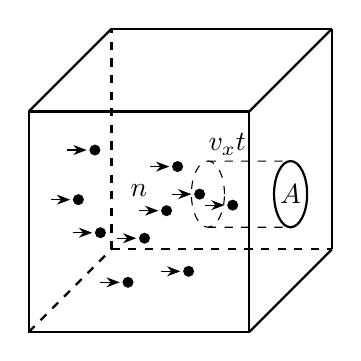
\begin{tikzpicture}[scale=0.7, >=Stealth]
                \def\L{4}
                \def\D{1.5}
                \coordinate (A) at (0,0);
                \coordinate (B) at (\L,0);
                \coordinate (C) at (\L,\L);
                \coordinate (D) at (0,\L);
                \coordinate (E) at (\D,\D);
                \coordinate (F) at (\L+\D,\D);
                \coordinate (G) at (\L+\D,\L+\D);
                \coordinate (H) at (\D,\L+\D);
                \draw[thick] (A)--(B)--(C)--(D)--cycle;
                \draw[thick] (B)--(F);
                \draw[thick] (C)--(G);
                \draw[thick] (D)--(H);
                \draw[thick] (F)--(G);
                \draw[thick] (G)--(H);
                \draw[thick,dashed] (A)--(E);
                \draw[thick,dashed] (E)--(F);
                \draw[thick,dashed] (E)--(H);
                \foreach \x/\y in {
                0.9/2.4, 1.2/3.3, 1.3/1.8, 1.8/0.9, 2.1/1.7,
                2.5/2.2, 2.7/3.0, 2.9/1.1, 3.1/2.5, 3.7/2.3
                }
                {
                \fill (\x,\y) circle (0.1);
                \draw[->] (\x-0.5,\y) -- (\x-0.15,\y);
                }
                \coordinate (front) at (\L+\D/2,\L/2+0.5);
                \draw[thick] (front) ellipse (0.3 and 0.6);
                \node at (front) {$A$};
                \coordinate (back) at ($(front)+(-1.5,0)$);
                \draw[dashed] (back) ellipse (0.3 and 0.6);
                \draw[dashed] ($(back)+(0,0.6)$) -- ($(front)+(0,0.6)$);
                \draw[dashed] ($(back)-(0,0.6)$) -- ($(front)-(0,0.6)$);
                \node at ($(back)+(0.35,0.9)$) {$v_x t$};
                \node[below=0.8cm] at (\L/2,\L) {$n$};
            \end{tikzpicture}
        \end{figure}
    \end{minipage}
\end{frame}

\begin{frame}{电子简并压的推导：非相对论情况}
    对于\textcolor{mari}{非相对论性电子：
    \[
        v = \frac{p_F}{m_e}
    \]
    }
    因此简并压为：
    \[
        P \sim n p_F \frac{p_F}{m_e} = \frac{n p_F^2}{m_e}
    \]
    代入$p_F \sim h n^{1/3}$，得到：
    \textcolor{mari}{
    \[
        P \sim \frac{n (h n^{1/3})^2}{m_e} = \frac{n h^2 n^{2/3}}{m_e} = \frac{h^2 n^{5/3}}{m_e}
    \]
    }
    因此，非相对论性电子简并压正比于\textcolor{dia}{电子密度的$\dfrac{5}{3}$次方}。
\end{frame}

\begin{frame}{电子简并压的推导：相对论情况}
    对于\textcolor{mari}{相对论性电子：
    \[
        v \approx c
    \]
    }
    因此简并压为：
    \[
        P \sim n p_F c
    \]
    代入$p_F \sim h n^{1/3}$，得到：
    \textcolor{mari}{
    \[
        P \sim n (h n^{1/3}) c = h c n^{4/3}
    \]
    }
    因此，相对论性电子简并压正比于\textcolor{dia}{电子密度的$\dfrac{4}{3}$次方}。
\end{frame}

\begin{frame}{电子简并压的推导：简并压与密度的关系}
    之前我们使用电子的数密度来表示简并压，但在实际应用中，我们更关心的是物质的质量密度$\rho$。电子数密度$n$与质量密度$\rho$之间的关系为：
    \[
        n = \frac{\rho}{\mu_e m_p}
    \]
    其中$\mu_e = A/Z$是每个电子对应的平均核子数，$m_p$是质子质量（忽略质子和中子的质量差和电子的质量）。对于一个一般由碳和氧组成的白矮星，$\mu_e \approx 2$，因此：
    \[
        n \approx \frac{\rho}{2 m_p}
    \]
    将这个关系代入之前的简并压表达式中，我们可以得到简并压与质量密度$\rho$的关系：
    \textcolor{dia}{
    \[
        P \sim \frac{h^2}{m_e} \left(\frac{\rho}{2 m_p}\right)^{5/3} \quad \text{（非相对论）},\quad
        P \sim h c \left(\frac{\rho}{2 m_p}\right)^{4/3} \quad \text{（相对论）}
    \]
    }
\end{frame}

\begin{frame}{电子简并压的推导：白矮星的质量——半径关系}
    对于白矮星，电子简并压是抵抗引力坍缩的主要机制。根据流体静力平衡方程：
    \textcolor{mari}{
    \[
        \frac{\Delta P}{\Delta r} = -\rho(r)g(r) = -\frac{G M(r) \rho(r)}{r^2}
    \]
    }
    对于一个质量为$M$、半径为$R$的白矮星，其中心压强可以估计为：
    \textcolor{mari}{
    \[
        \frac{P}{R} \sim \frac{G M \rho}{R^2} \implies P \sim \frac{G M \rho}{R} \sim \frac{G M^2}{R^4}
    \]
    }
    下面我们将这个表达式与之前的简并压表达式进行比较，估计白矮星的质量——半径关系。
\end{frame}

\begin{frame}{电子简并压的推导：白矮星的质量——半径关系}
    非相对论情况：
    \[
        P \sim \frac{h^2}{m_e} \left(\frac{\rho}{2 m_p}\right)^{5/3} \propto \rho^{5/3}
    \]
    即：
    \textcolor{mari}{
    \[
        P \propto \left(\frac{M}{R^3}\right)^{5/3} = \frac{M^{5/3}}{R^5}
    \]
    }
    将此表达式代入中心压强表达式中：（$k$为比例常数）
    \[
        \frac{G M^2}{R^4} = k \frac{M^{5/3}}{R^5}
    \]
    整理得：
    \textcolor{dia}{
    \[
        R \sim M^{-1/3}
    \]
    }
    这说明，白矮星的质量越大，半径反而越小。
\end{frame}

\begin{frame}{电子简并压的推导：钱德拉塞卡极限}
    相对论情况：
    \[
        P \sim h c \left(\frac{\rho}{2 m_p}\right)^{4/3} \propto \rho^{4/3}
    \]
    即：
    \textcolor{mari}{
    \[
        P \propto \left(\frac{M}{R^3}\right)^{4/3} = \frac{M^{4/3}}{R^4}
    \]
    }
    将此表达式代入中心压强表达式中：（$k$为比例常数）
    \[
        \frac{G M^2}{R^4} = k \frac{M^{4/3}}{R^4}
    \]
    整理得：
    \textcolor{dia}{
    \[
        M = k^{3/2} G^{-3/2} = \mathrm{const.}
    \]
    }
    这说明，在相对论极限下，白矮星的质量达到一个临界值时，无法再通过增加质量来维持平衡，这个临界值被称为\textcolor{dia}{钱德拉塞卡极限}，约为\textcolor{dia}{$1.44 M_\odot$}。
\end{frame}

\section{中子星}

\begin{frame}{中子星}
    当恒星的核心质量超过了钱德拉塞卡极限时，电子简并压将无法抵抗引力，核心继续坍缩，直到质子和电子因引力作用结合在一起成为中子，形成\textcolor{dia}{中子星}。中子星的半径在$10\,\mathrm{km}$左右，因此中子星的密度极高，通常在$10^{14} \sim 10^{15}\,\mathrm{g/cm^3}$的范围。

    中子和电子一样，也是遵循泡利不相容原理的费米子，因此这些中子在一起产生的\textcolor{mari}{中子简并压}，可以抗衡引力使得恒星成为密度比白矮星大得多的稳定的中子星。

    类似于白矮星的钱德拉塞卡极限，中子星的质量极限是\textcolor{mari}{托尔曼-奥本海默-沃尔科夫极限（TOV极限），约为$2 \sim 3 M_\odot$}，超过这个质量的中子星将无法维持稳定，最终坍缩成黑洞。
\end{frame}

\begin{frame}{中子简并压}
    中子简并压的推导与电子简并压类似，但需要考虑中子的质量和相互作用。中子简并压的表达式可以表示为：
    \textcolor{mari}{
    \[
        P \sim \frac{h^2}{m_n} n_n^{5/3} = h^2 \frac{\rho^{5/3}}{m_n^{8/3}}
    \]
    }
    其中$m_n$是中子质量，$n_n$是中子数密度。由于中子的质量远大于电子，因此\textcolor{mari}{中子简并压在相同密度下比电子简并压更大}，这也是为什么中子星能够抵抗更大的引力而不坍缩成黑洞。
\end{frame}

\section{黑洞}

\begin{frame}{黑洞的形成}
    当恒星的核心质量超过TOV极限时，中子简并压也无法抵抗引力，核心继续坍缩，最终形成\textcolor{dia}{黑洞}。

    黑洞是一种引力极强的天体，其引力场强大到连光都无法逃脱。黑洞的边界称为\textcolor{dia}{事件视界}，\textcolor{mari}{一旦物质或辐射进入事件视界，就无法再逃逸出来}。

    黑洞的形成过程涉及到极端的物理条件和复杂的相对论效应，目前仍是天体物理学中的一个重要研究领域。
\end{frame}

\begin{frame}{黑洞：史瓦西半径}
    最简单的黑洞模型是\textcolor{dia}{史瓦西黑洞}，它是一个球对称、非旋转、无电荷的黑洞，其视界半径为\textcolor{dia}{史瓦西半径$r_s$}。一个质量为$M$的物体，如果压缩到$r_s$以内，就会不断坍缩成一个奇点。史瓦西半径的表达式为：
    \textcolor{dia}{
    \[
        r_s = \frac{2GM}{c^2}
    \]
    }
    其中$G$是引力常数，$M$是物体的质量，$c$是光速。

    史瓦西半径的严格推导需要用到广义相对论，但这个公式提供了一个简单的方式来估计黑洞的大小：考虑一个光子在质量为$M$、半径为$R$的物体表面上以光速运动，其逃逸速度为
    \[
        v_\mathrm{esc} = \sqrt{\frac{2GM}{R}}
    \]
    \textcolor{mari}{如果逃逸速度等于光速$c$，那么这个半径就是史瓦西半径}。太阳的史瓦西半径约为$3\,\mathrm{km}$。
\end{frame}

\section{超新星}

\begin{frame}{超新星}
    \textcolor{dia}{超新星}是大质量恒星在演化接近末期时经历的一种剧烈爆炸。超新星爆发与白矮星、中子星和黑洞密切相关。

    超新星可以由两种方式触发：\textcolor{mari}{重新点燃核聚变的白矮星（Ia型超新星），或是大质量恒星核心的重力坍缩（Ib/Ic/II型超新星）}。

    需要注意的是，超新星的分类原本是根据\textcolor{mari}{光谱}而非来源分类的。I型超新星与II型超新星的区别是光谱中\textcolor{mari}{是否存在氢线}。I型超新星没有氢线，II型超新星有明显的氢线。这是因为I型超新星的前身是失去外层氢包层的恒星，而II型超新星的前身则保留了氢包层。Ia型超新星在亮度接近峰值时只呈现单一的硅（Si II）谱线，而Ib/Ic型超新星则没有这个谱线。
\end{frame}

\begin{frame}{超新星：Ia型超新星}
    \textcolor{mari}{如果双星系统中的一颗CO白矮星从伴星处吸积到足够的质量，达到钱德拉塞卡极限，它将不再能以电子简并压力支撑引力，并且开始坍缩。}在几秒钟内，白矮星相当大一部分的物质会发生核聚变，释放出足够的能量来摧毁整个恒星，形成\textcolor{dia}{Ia型超新星}。

    另一种Ia超新星的爆炸涉及两颗白矮星的合并，加起来的质量可能超过钱德拉塞卡极限，最终导致爆炸。

    正常Ia超新星光度曲线的峰值是非常一致的，最大值是\textcolor{mari}{绝对星等$-19.3\,\mathrm{mag}$}，这使它能成为宇宙距离的\textcolor{dia}{标准烛光}。
\end{frame}

\begin{frame}{超新星：中心坍缩超新星}
    另一种超新星的形成类型涉及大质量恒星（$M > 8 M_\odot$）的核心坍缩。

    \textcolor{mari}{当大质量恒星的核聚变无法克服自身引力维持核心结构时，会发生核心坍缩。}这是除了Ia型超新星之外，其它所有类型的超新星形成的原因。这种崩溃的结果会导致恒星的外层剧烈爆炸，成为超新星。恒星的内部最后会形成一个中子星或黑洞，取决于核心的质量。

    这产生了\textcolor{dia}{II型超新星}（保留厚氢包层，对应于典型红超巨星）和\textcolor{dia}{Ib/Ic型超新星}（失去厚氢包层，对应于被强恒星风剥离的沃尔夫——拉叶星或双星质量转移后被剥离的恒星）。
\end{frame}

\begin{frame}[plain]
    \begin{center}
        \huge
        \textbf{谢谢大家！}
    \end{center}
\end{frame}

\end{document}
